\colorbox{white!10!}{
    \begin{minipage}{0.2\textwidth}
       \begin{flushleft}
        \includegraphics[width = 0.6\textwidth]{Эмблема.png}
       \end{flushleft}
    \end{minipage}
    \begin{minipage}[t]{0.7 \textwidth}
        \begin{center}
            {\huge \textsc{Красноярская Летняя Школа. Сезон $7^2 - 2$}}
            \vspace{0.25cm}
            
            { \huge \textbf{ФМТ. Тур 2.}}
        \end{center}
        \vspace{0.05cm}
    \end{minipage}
}

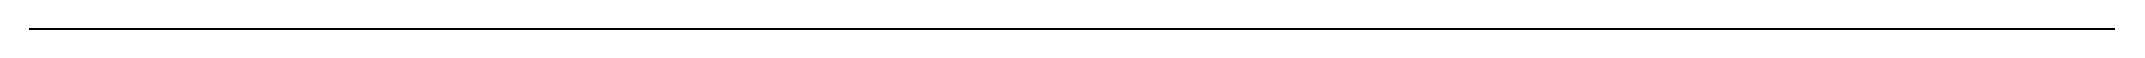
\begin{tikzpicture}
    \draw[thick] (-6.5,0)--(20,0);
\end{tikzpicture}
\begin{enumerate}
    \item Через какое время после включения закипит вода в электрическом чайнике мощностью 600 Вт? Масса воды $m = 2$ кг, её начальная температура $t = 20^{o}$ С, КПД чайника $50 \%$.
	\item Стальной кубик с длиной ребра $а$ плавает в жидкости с плотностью $\rho_1$. Поверх первой жидкости наливают жидкость с плотностью $\rho_2$ вровень с верхней гранью кубика. Какова высота $h$ слоя второй жидкости, если $\rho_1>\rho_2$?

\end{enumerate}